\section*{\centering XL Международная олимпиада школьников по физике}
\begin{multicols*}{2}
    \footnotesize В этом году Международная физическая олимпиада (МФО) школьников проходила в Мексике, в городе Мерида. Из-за тревожной эпидемиологической обстановки в этой стране часть команд отказалась от участия в олимпиаде. В Мериду прибыли только 316 школьников из 69 стран (для сравнения - в прошлом году во Вьетнаме было 376 участников из 76 государств).
    
    В сборную команду России вошли:
    
    \textit{Трегубов Дмитрий} - Киров, ФМЛ, учителя-наставники Канин Павел Евгеньевич, Гырдымов Михаил Владимирович,
    
    \textit{Землянов Владислав} - Урай (Ханты-Мансийский автономный округ), гимназия, учитель-наставник Козловская Зоя Георгиевна,
    
    \textit{Кудряшова Нина} - Бийск, Бийский лицей Алтайского края, учитель-наставник Аполонский Александр Николаевич,
    
    \textit{Дорошенко Андрей} - Омск, лицей 92, учитель-наставник Афанасьева Юлика Александровна,
   
    \textit{Старков Григорий} - Ноябрьск (Ямало-Ненецкий автономный округ), школа 7, учитель-наставник Ткачук Игорь Викторович.
    
    Команду России возглавили профессор Московского физико-технического института (МФТИ) Станислав Миронович Козел и доцент МФТИ Валерий Павлович Слободянин. В составе российской делегации в качестве наблюдателя работал доцент МФТИ Михаил Николаевич Осин.
    
    Как и в прошлые годы, восемь кандидатов в команду России были приглашены на последние трехнедельные летние сборы, на которых отрабатывались навыки экспериментальной работы на сложном современном оборудовании и дополнительно изучались элементы специальной теории относительности, волновой оптики, ядерной физики и ряд других тем, входящих в программу МФО. Во время сборов с командой работали преподаватели кафедры общей физики МФТИ, СУНЦ МГУ, научные сотрудники институтов Российской академии наук, а также студенты Физтеха - победители Международных физических олимпиад прошлых лет.
    
    \begin{center}
        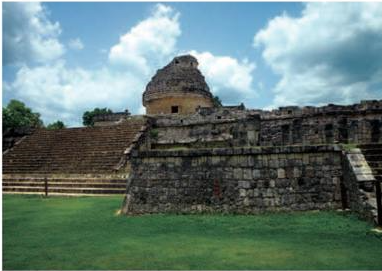
\includegraphics[width=0.48\textwidth]{observatory.png}
    \end{center}
    \textit{Обсерватория майя (Мексика)}
    
    
    \columnbreak

    \begin{center}
        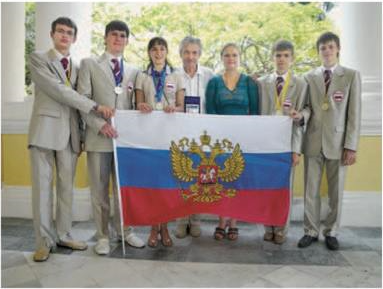
\includegraphics[width=0.48\textwidth]{team.png}
    \end{center}
    \textit{Команда России на XL МФО. Слева направо: Г.Старков, А.Дорошенко, Н.Кудряшова, С.М.Козел, Маша - гид нашей команды, В.Землянов, Д.Трегубов}

    \vspace{10pt}

    На олимпиаде участникам были предложены три теоретические задачи и два экспериментальных задания. Каждая задача и каждое задание оценивались из 10 баллов. Таким образом, максимальное количество баллов, которое мог набрать каждый из участников олимпиады, равнялось 50.

    Оба тура олимпиады - теоретический и экспериментальный - оказались крайне трудоемкими. Ниже приведен список из 11 лидирующих стран (согласно их рейтингу):
    \begin{center}
        \begin{tabular}{clcccp{1.5cm}cc}
            № & Страна & \multicolumn{3}{c}{Количество медалей} & Сумма баллов \\
             & & золото & серебро & бронза & \\
             1 & Китай & 5 & & & 216 \\
             2 & Корея & 4 & 1 & & 186 \\
             3 & Индия & 4 & 1 & & 180 \\
             4 & Тайвань & 3 & 2 & & 179 \\
             5 & США & 4 & 1 & & 176 \\
             6 & Россия & 3 & 2 & & 165 \\
             7 & Румыния & 3 & 2 & & 161 \\
             8 & Сингапур & 2 & 3 & & 154 \\
             9 & Таиланд & 1 & 4 & & 152 \\
             10 & Индонезия & 1 & 3 & 1 & 148 \\
             11 & Япония & 2 & 1 & 2 & 144 \\
        \end{tabular}
    \end{center}

    Как видно из таблицы, лидерство на олимпиаде захватили страны из Юго-Восточной Азии. Команды этих стран устойчиво добиваются высоких результатов в Международных олимпиадах и по другим предметам.

    Члены сборной России показали следующие результаты:
    \begin{center}
        \begin{tabular}{p{1.9cm}p{1.3cm}p{2cm}p{1.1cm}p{2cm}c}
             Участник & Теория & Эксперимент & Сумма баллов & \centering{Медаль} & \\
             Старков Григорий & \centering{21,45} & \centering{14,00} & \centering{35,45} & \centering{золото} & \\
             
             Землянов Владислав & \centering{20,60} & \centering{13,65} & \centering{34,75} & \centering{золото} & \\
             
        \end{tabular}
    \end{center}
\end{multicols*}

\section*{\centering Логарифмические уравнения}
\flushright \textbf{В. В. Гольдберг}

\jjЛогарифмическими уравнениями принято называть уравнения, содержащие неизвестную величину под знаком логарифма.

Решение простейшего логарифмического уравнения
\begin{equation}
    \log_af(x)=b
\end{equation}
основано на следующем свойстве логарифмов: \textit{если логарифмы двух (положительных) чисел по одному и тому же основанию $a(a>0, a\neq1)$ равны, то равны и сами эти числа}.

Записав уравнение (1) в виде $\log_ax=\log_aa^b$ и воспользовавшись указанным свойство, получим ответ: $x=a^b$.

Этот прием применим и для решения более сложных логарифмических уравнений вида
\begin{equation}
    \log_af(x)=b
\end{equation}
Для уравнения (2) получаем $f(x)=a^b$.

П р и м е р 1. \textit{Решить уравнение}
\begin{equation*}
    \log_5[2+\log_3(3+x)]=0
\end{equation*}

Р е ш е н и е. Сначала получаем, что
\begin{equation*}
    2+\log_3(3+x)=5^0, 2+\log_3(3+x)=1,\log_3(3+x)=-1
\end{equation*}